\documentclass[a4paper,14pt]{extarticle}

\usepackage[utf8x]{inputenc}
\usepackage[T1]{fontenc}
\usepackage[russian]{babel}
\usepackage{hyperref}
\usepackage{indentfirst}
\usepackage{here}
\usepackage{array}
\usepackage{graphicx}
\usepackage{caption}
\usepackage{subcaption}
\usepackage{chngcntr}
\usepackage{amsmath}
\usepackage{amssymb}
\usepackage[left=2cm,right=2cm,top=2cm,bottom=2cm,bindingoffset=0cm]{geometry}
\usepackage{multicol}
\usepackage{multirow}
\usepackage{titlesec}
\usepackage{listings}
\usepackage{color}
\usepackage{enumitem}
\usepackage{cmap}
\usepackage{url}

\definecolor{green}{rgb}{0,0.6,0}
\definecolor{gray}{rgb}{0.5,0.5,0.5}
\definecolor{purple}{rgb}{0.58,0,0.82}

\lstdefinelanguage{none}{}

\lstset{
	language={none},
	inputpath={../logs/},
	backgroundcolor=\color{white},
	commentstyle=\color{green},
	keywordstyle=\color{blue},
	numberstyle=\color{gray}\scriptsize\ttfamily,
	stringstyle=\color{purple},
	basicstyle=\footnotesize\ttfamily,
	breakatwhitespace=false,
	breaklines=true,
	captionpos=b,
	keepspaces=true,
	numbers=left,
	numbersep=5pt,
	showspaces=false,
	showstringspaces=false,
	showtabs=false,
	tabsize=4,
	frame=single,
	morekeywords={},
	deletekeywords={},
	extendedchars=false,
	columns=fullflexible,
	literate=%
		{~}{{\raise.25ex\hbox{$\mathtt{\sim}$}}}{1}%
		{-}{-}{1}
}

\titleformat*{\section}{\large\bfseries} 
\titleformat*{\subsection}{\normalsize\bfseries} 
\titleformat*{\subsubsection}{\normalsize\bfseries} 
\titleformat*{\paragraph}{\normalsize\bfseries} 
\titleformat*{\subparagraph}{\normalsize\bfseries} 

\counterwithin{figure}{section}
\counterwithin{equation}{section}
\counterwithin{table}{section}
\newcommand{\sign}[1][5cm]{\makebox[#1]{\hrulefill}}
\newcommand{\equipollence}{\quad\Leftrightarrow\quad}
\newcommand{\no}[1]{\overline{#1}}
\graphicspath{{../pics/}}
\captionsetup{justification=centering,margin=1cm}
\def\arraystretch{1.3}
\setlength\parindent{5ex}
\titlelabel{\thetitle.\quad}

\setitemize{topsep=0em, itemsep=0em}
\setenumerate{topsep=0em, itemsep=0em}

\begin{document}

\begin{titlepage}
\begin{center}
	Санкт-Петербургский Политехнический Университет Петра Великого\\[0.3cm]
	Институт компьютерных наук и технологий \\[0.3cm]
	Кафедра компьютерных систем и программных технологий\\[4cm]
	
	\textbf{ОТЧЕТ}\\ 
	\textbf{по лабораторной работе}\\[0.5cm]
	\textbf{<<Data Mining>>}\\[0.1cm]
	Интеллектуальные системы\\[3.0cm]
\end{center}

\begin{flushright}
	\begin{minipage}{0.5\textwidth}
		\textbf{Работу выполнил студент}\\[3mm]
		гр. 3540901/91502 \hfill \sign[1.1cm] \hfill Дьячков В.В.\\[5mm]
		\textbf{Работу принял преподаватель}\\[5mm]
		\sign[2.1cm] \hfill к.т.н., доц. Бендерская Е.Н. \\[5mm]
	\end{minipage}
\end{flushright}

\vfill

\begin{center}
	Санкт-Петербург\\[0.3cm]
	\the\year
\end{center}
\end{titlepage}

\addtocounter{page}{1}

\tableofcontents
\newpage

\section{Программа работы}

\begin{enumerate}
	\item Приведите интенсиональное и экстенсиональные определения двух понятий на ваш выбор.
	\item Постройте ментальную модель знаний в предметной области по вашему выбору с помощью интеллект-карты, которая будет содержать не менее четырех уровней ветвления\footnote{\url{http://www.mind-map.ru}}.
	\item Разработайте стратегию принятия решений о приеме на работу кандидата в выбранную Вами компанию и записать решение в виде:
	\begin{itemize}
		\item набора продукционных правил \footnote{\url{http://itteach.ru/predstavlenie-znaniy/produktsionnaya-modelpredstavleniya-znaniy}}
		\item дерева принятия решений  \footnote{\url{http://logic.pdmi.ras.ru/~sergey/teaching/ml/notes-01-dectrees.pdf}}
		\item таблицы решений \footnote{\url{http://5fan.ru/wievjob.php?id=14722}}
	\end{itemize}
	\item Выделите отличия и сходства следующих моделей представления знаний: логических, сетевых, продукционных и сценарий. Постарайтесь дать объяснения этим различиям.
	\item Что такое онтологии, деревья, фреймы? В чем сходство и различие данных моделей?
	\item Ознакомьтесь с теорией экспертных систем (ЭС). Опишите различие между базой данных (БД) и базой знаний (БЗ). Что такое логика предикатов? Что такое «правило вывода»? В чем сильные и слабые стороны любой ЭС?
	\item Приведите не менее 3 примеров экспертных систем в каждой из предметных областей, разработанную в последнее десятилетие (не позднее 2009).
\end{enumerate}

\newpage

\section{Выполнение работы}

\subsection{Интенсиональное и экстенсиональные определения}

\textbf{Интенсионал} -- это термин, обозначающий содержание слова-понятия, то есть совокупность мыслимых признаков обозначаемого данным понятием предмета. 

\textbf{Экстенсионал} -- это термин, обозначающий объём слова-понятия, то есть совокупность обозначаемых данным понятием предметов.\\

Пример определений:
\begin{itemize}
	\item[\emph{Инт.}] \textbf{Растение} включает в себя такие свойства, как «состоять из целлюлозы», «живой», «организм» и др. \cite{intension}
	\item[\emph{Экст.}]  \textbf{Собака} -- это набор всех (прошлых, настоящих и будущих) собак в мире: набор включает в себя Фидо, Ровер, Лэсси, Рекс и так далее. \cite{extension} \\
\end{itemize}

Пример высказываний:
\begin{itemize}
	\item[\emph{Инт.}] Каждый, кто читал Гекльберри Финна, знает, что это написал Марк Твен.
	\item[\emph{Экст.}] Марк Твен написал Гекльберри Финн.
\end{itemize}

\subsection{Интеллект-карта}

\begin{figure}[H]
	\centering
	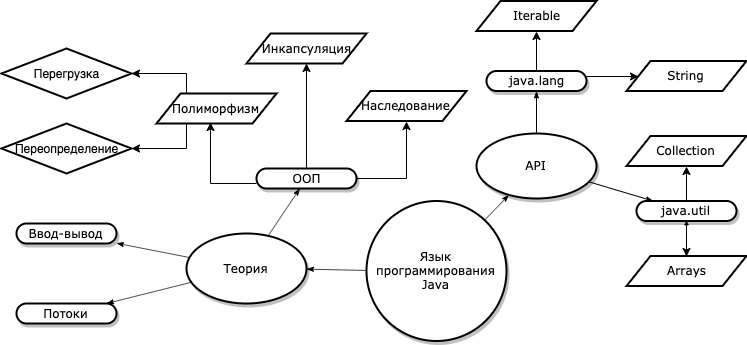
\includegraphics[width=\linewidth]{java.png}
	\caption{Интеллект-карта для языка программирования Java}
	\label{fig:my_label}
\end{figure}

\subsection{Стратегия принятия решений}

\subsubsection{Набор продукционных правил}

\begin{enumerate}
	\item Если у кандидата есть прописка в Санкт-Петербурге, то переходим к пункту 2, иначе кандидат нам не подходит.

	\item Если у кандидата есть высшее образование в Computer Science, то переходим к шагу 3, иначе кандидат нам не подходит.

	\item Если кандидат может ответить на все вопросы про язык программирования Java, то переходим к шагу 4, иначе кандидат нам не подходит.

	\item Если кандидат имеет опыт работы с фреймворком Spring, то мы его принимаем в нашу компанию, иначе переходим к шагу 5.

	\item Если кандидат готов работать за еду, то мы его принимаем в нашу компанию, иначе кандидат нам не подходит.
\end{enumerate}

\subsubsection{Дерево принятия решений}

\begin{figure}[H]
	\centering
	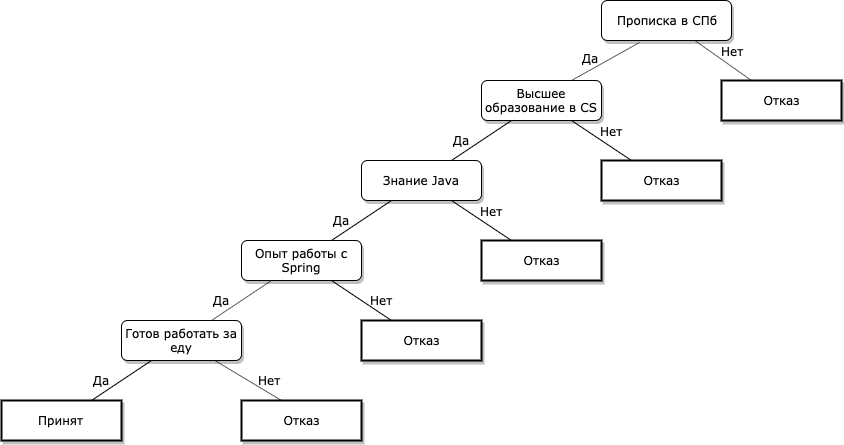
\includegraphics[width=\linewidth]{interview.png}
	\caption{Дерево принятия решений о приеме на работу}
	\label{fig:my_label}
\end{figure}

\subsubsection{Таблица решений}

\begin{table}[H]
	\def\tabcolsep{12pt}
	\caption{Таблица решений о приеме на работу}
	\begin{tabular}{|c|c|c|c|c|c|c|}
	\hline
	Прописка в СПб		  & Нет & Да  & Да  & Да  & Да  & Да  \\ \hline
	Высшее образование в CS & $-$ & Нет & Да  & Да  & Да  & Да  \\ \hline
	Знание Java			 & $-$ & $-$ & Нет & Да  & Да  & Да  \\ \hline
	Опыт работы с Spring	& $-$ & $-$ & $-$ & Нет & Да  & Да  \\ \hline
	Готов работать за еду   & $-$ & $-$ & $-$ & $-$ & Нет & Да  \\ \hline
	\textbf{Отказ}		  & $+$ & $+$ & $+$ & $-$ & $+$ &	 \\ \hline
	\textbf{Принят}		 &	 &	 &	 &	 &	 & $+$ \\ \hline
	\end{tabular}
\end{table}

\subsection{Модели представления знаний}

\begin{itemize}
	\item \textbf{Продукционные модели} -- модели основанные на правилах, позволяют представить знание в виде предложений типа: «ЕСЛИ условие, ТО действие». Продукционные модели обладает тем недостатком, что при накоплении достаточно большого числа правил, они начинают противоречить друг другу \cite{air-models}.
	
	\item \textbf{Сетевые модели} (семантические сети) -- как правило, это граф, отображающий смысл целостного образа. Узлы графа соответствуют понятиям и объектам, а дуги – отношениям между объектами \cite{air-models}.
	
	\item \textbf{Сценарием} называется формализованное описание стандартной последовательности взаимосвязанных фактов, определяющих типичную ситуацию предметной области. Это могут быть последовательности действий или процедур, описывающие способы достижения целей действующих лиц сценария (например: обед в ресторане, командировка, полет самолета, поступление в вуз). В интеллектуальных системах сценарии используются в процедурах понимания естественно-языковых текстов, планирования поведения, обучения, принятия решений, управления изменениями среды и др. \cite{scenario}
	
	\item \textbf{Логические модели} -- информация, необходимая для решения прикладных задач, рассматривается как совокупность фактов и утверждений, которые представляются как формулы в некоторой логике. Знания отображаются совокупностью таких формул, а получение новых знаний сводится к реализации процедур логического вывода. Для логических моделей существуют достаточно эффективные процедуры вывода, в том числе реализованные в языке логического программирования «Пролог» \cite{logic-models}.
\end{itemize}

У каждой модели существуют свои достоинства и недостатки. Каждый тип модели применим в определенных условиях, например продукционные модели чаще подходят для небольшого числа правил. Логические модели позволяют использовать аппарат математической логики, которые хорошо проработаны и изучены. Представление модели в виде сценария позволяет восстанавливать информацию, пропущенную в описании ситуации, предсказывать появления новых фактов, которых можно ожидать в данной ситуации.

\subsection{Представление знаний}

\begin{itemize}
	\item \textbf{Онтология} –- это попытка всеобъемлющей и детальной формализации некоторой области знаний с помощью концептуальной схемы. Обычно такая схема состоит из иерархической структуры данных, содержащей все релевантные классы объектов, их связи и правила (теоремы, ограничения), принятые в этой области.
	
	\item \textbf{Фрейм} –- структура данных для представления некоторого концептуального объекта. Информация, относящаяся к фрейму, содержится в составляющих его слотах. Слоты могут быть терминальными либо являться сами фреймами, т.о. образуя целую иерархическую сеть.
	
	\item \textbf{Деревом решений} называют графическое представление модели знаний, которое объединяет все ветви поиска для вершины определенного типа базируясь на знаниях эксперта \cite{tree}.
\end{itemize}

На сегодняшний день разработано большое количество моделей и каждая из них обладает своими плюсами и минусами, и поэтому для каждой конкретной задачи необходимо выбрать именно свою модель. От этого будет зависит не столько эффективность выполнения поставленной задачи, сколько возможность ее решения вообще.

\subsection{Теория экспертных систем}

\begin{itemize}
	\item \textbf{База знаний} (БЗ) отличается от \textbf{базы данных} (БД) тем, что полноценные базы знаний содержат в себе не только фактическую информацию, но и правила вывода, позволяющие делать автоматические умозаключения об уже имеющихся или вновь вводимых фактах и тем самым производить семантическую (осмысленную) обработку информации \cite{knowledge-base}.
	
	\item \textbf{Логика предикатов} -- это раздел символической логики, изучающий рассуждения и другие языковые контексты с учётом внутренней структуры входящих в них простых высказываний, при этом выражения языка трактуются функционально, то есть как знаки некоторых функций или же как знаки аргументов этих функций.
	
	\item \textbf{Правило вывода} -- эффективная процедура для проверки того, что одна заданная формула в рассматриваемой теории непосредственно за один шаг выводится из других заданных формул.
	
	\item \textbf{Достоинства} экспертных систем \cite{kb-pros}:
		\begin{enumerate}
			\item Постоянство. Человеческая компетенция ослабевает со временем. Перерыв в деятельности человека-эксперта может серьёзно отразиться на его профессиональных качествах.

			\item Лёгкость передачи.

			Передача знаний от одного человека другому – долгий и дорогой процесс. Передача искусственной информации – это простой процесс копирования программы или файла данных.

			\item Устойчивость и воспроизводимость результатов.

			Экспертные системы устойчивы к «помехам». Человек же легко поддается влиянию внешних факторов, которые непосредственно не связаны с решаемой задачей. Эксперт-человек может принимать в тождественных ситуациях разные решения из-за эмоциональных факторов. Результаты экспертной системы – стабильны.

			\item Стоимость.

			Эксперты, особенно высококвалифицированные обходятся очень дорого. Экспертные системы, наоборот, сравнительно недороги. Их разработка дорога, но они дёшевы в эксплуатации.
		\end{enumerate}
		
		\item \textbf{Недостатки} экспертных систем \cite{kb-cons}:
			\begin{enumerate}
				\item Здравый смысл. В дополнение к широкому техническому знанию, человек-эксперт имеет здравый смысл. Еще не известно, как заложить здравый смысл в экспертные системы.
				
				\item Творческий потенциал. Человек-эксперт может реагировать творчески на необычные ситуации, экспертные системы не могут.
				
				\item Обучение. Человек-эксперт автоматически адаптируются к изменению среды; экспертные системы нужно явно модифицировать.
				
				\item Сенсорный опыт. Человек-эксперт располагает широким диапазоном сенсорного опыта; экспертные системы в настоящее время основаны на вводе символов.
			\end{enumerate}
\end{itemize}

\newpage

\subsection{Примеры экспертных систем}

Приведем примеры экспертных систем \cite{examples-1}, \cite{examples-2}.

\begin{table}[H]
	\def\tabcolsep{12pt}
	\begin{tabular}{|c|c|c|}
	\hline
	\textbf{Предметная область} & \textbf{Название, страна, год} & \textbf{Ссылка} \\ \hline
	Геология & DIPMETER ADVISOR, США, 1980 & \href{http://en.wikipedia.org/wiki/Dipmeter\_Advisor}{Ссылка} \\ \hline
	 & PROSPECTOR, США, 1974-1983 & \href{https://tpl-it.wikispaces.com/PROSPECTOR}{Ссылка} \\ \hline
	 & Litho, Россия & \href{http://gisistem.ucoz.ru/index/0-7}{Ссылка} \\ \hline
	Юриспруденция & SHYSTER, Австралия, 2003 & \href{https://en.wikipedia.org/wiki/Shyster_%28expert_system%29}{Ссылка}  \\ \hline
	 & JUDITH, Германия 1975 & \href{http://www.inteltec.ru/publish/articles/textan/expertm2.shtml}{Ссылка} \\ \hline
	 & LEGAL ANALYSIS SYSTEM, США & \href{http://www.inteltec.ru/publish/articles/textan/expertm2.shtml}{Ссылка} \\ \hline
	Медицина & MYCIN, США & \href{http://expro.ksu.ru/materials/ii_i_es/book.html#point1.6}{Ссылка} \\ \hline
	 & CASNET-EXPERT, США & \href{http://expro.ksu.ru/materials/ii_i_es/book.html#point1.6}{Ссылка} \\ \hline
	 & REPER, Россия & \href{http://www.inteltec.ru/publish/articles/textan/expertm2.shtml}{Ссылка} \\ \hline
	Экономика & FLiPSiDE, США & \href{http://www.tora-centre.ru/library/razn/finan.htm}{Ссылка} \\ \hline
	 & Splendors, США & \href{http://www.tora-centre.ru/library/razn/finan.htm}{Ссылка} \\ \hline
	 & Le Courtier, США & \href{http://www.tora-centre.ru/library/razn/finan.htm}{Ссылка} \\ \hline
	Биология & META-DENDRAL, США, 1965 & \href{http://sapr.mgsu.ru/biblio/ex-syst/Glava20/Index3.htm}{Ссылка} \\ \hline
	 & MOLGEN, Германия, 1985 & \href{http://www.molgen.de/}{Ссылка} \\ \hline
	 & GENESIS, США & \href{http://chernykh.net/content/view/196/208/}{Ссылка} \\ \hline
	\end{tabular}
\end{table}

\newpage

\bibliographystyle{plain}
\addcontentsline{toc}{section}{Список литературы}
\bibliography{refs}

\end{document}